\section{Задание 3. Аналитическое задание множества.}

\textbf{Условие.}

Определите траекторию точки, которая в своем движении остается вдвое ближе к
точке $A(1,0)$, чем к точке $B(4,0)$.

\begin{enumerate}
    \item Сделайте иллюстрацию к условию задачи: введите удобную для решения систему
координат, необходимые обозначения, подпишите известные величины и
соотношения.
    \item Во введенных обозначениях запишите геометрическое свойство множества, для
которого ищется уравнение.
    \item Сведите геометрическое свойство к уравнению.
    \item Изобразите множество по его уравнению.
\end{enumerate}
\vspace{10mm}
\textbf{Решение.}

Введём декартову прямоугольную систему координат.

Определим функцию $Distance(a, b)$ как растояние на плоскости между двумя точками: a и b:

$Distance(a, b) = \sqrt{(a_x - b_x)^2 + (a_y - b_y)^2}$

Таким образом ГМТ в ПДСК выглядит как: $\Set{c \mid 2*Distance(A, c) = Distance(B, c)}$, где $c$ -  точка на траектории заданного движения.

Или через отношения: $\cfrac{Distance(B, c)}{Distance(A, c)} = 2$

Пусть у точки $c$ координаты $(x, y)$, тогда:

\vspace{1mm}

$\displaystyle \frac{\sqrt{(x-B_x)^2 + (y - B_y)^2}}{\sqrt{(x-A_x)^2 + (y-A_y)^2}} = 2$\\
\vspace{1mm}

$\sqrt{(x-B_x)^2 + (y - B_y)^2} = 2 \sqrt{(x-A_x)^2 + (y-A_y)^2}$

Т.к. под корнем сумма квадратов, то подкоренное выражениеи всегда положительно, т.е. можно равноильно возвести в квадрат:

$(x-B_x)^2 + (y - B_y)^2 = 4 ((x-A_x)^2 + (y-A_y)^2)$

$x^2 - 2B_xx + {B_x}^2 + y^2 - 2B_yy + {B_y}^2 = 4 (x^2 - 2A_xx + {A_x}^2 + y^2 - 2A_yy + {A_y}^2)$

$x^2 - 2B_xx + {B_x}^2 + y^2 - 2B_yy + {B_y}^2 = 4x^2 - 8A_xx + 4{A_x}^2 + 4y^2 - 8A_yy + 4{A_y}^2$

$x^2 - 8x + 16 + y^2 = 4x^2 - 8x + 4 + 4y^2$

$12 = 3x^2 + 3y^2$

$4 = x^2 + y^2$

$\cfrac{x^2}{2^2} + \cfrac{y^2}{2^2} = 1$

Это же буквально каноническое уравнене элипса вид

$\cfrac{x^2}{a^2} + \cfrac{y^2}{b^2} = 1$

где $a$ и $b$ = 2.

Т.е. это еще и круг. с центром в $(0, 0)$

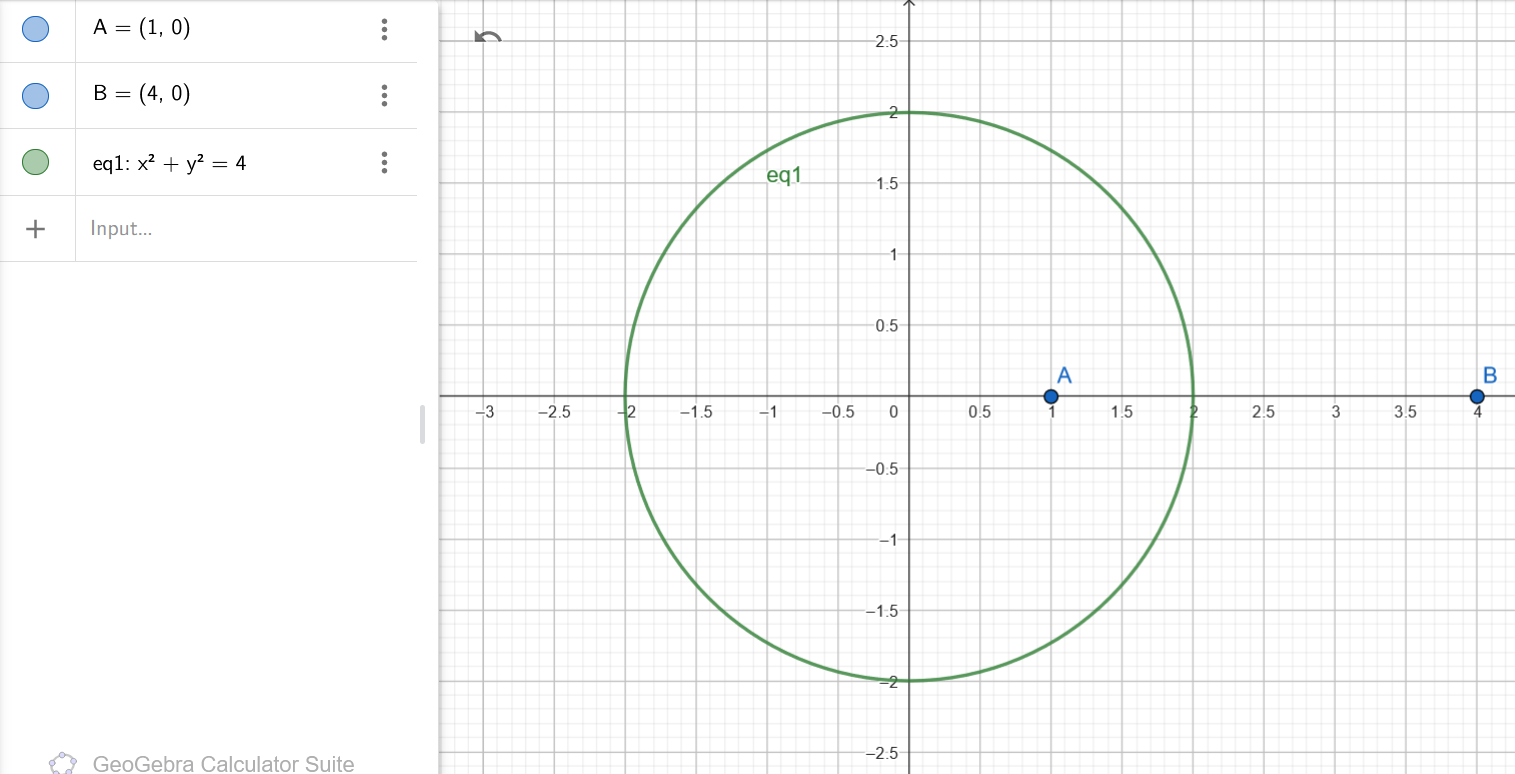
\includegraphics[width=0.9\linewidth]{images/3_ball.png}

\clearpage
